\documentclass[12pt]{article}
\usepackage[margin=0.75in]{geometry}
\usepackage{graphicx}
\usepackage{multicol}
\usepackage{float}
\usepackage{upgreek}
\usepackage{amsmath}

% for dots in TOC:
\usepackage{tocloft}
\renewcommand{\cftsecleader}{\cftdotfill{\cftdotsep}}

\setlength{\parindent}{0mm}

\begin{document}

{\centering
\LARGE Physics I-II Lab Manual \par
}
\hfill \break

{\centering
\large Preface \par
}
\hfill \break \vspace{-4mm}

This is the lab manual for Physics 2211L, 2212L, 1111L, and 1112L taught by Dr. Nathan Harrison.
In some labs you will have to copy and paste small amounts of code;
it is recommended that you copy from the the original \LaTeX \ source, \textit{not} from the PDF file which often leads to formatting errors.
Another common mistake is to not unzip the Java-based simulations;
if the simulation opens but the screen is blank it is because you didn't unzip the file.
\vfill
\textcopyright \ Nathan Harrison 2018
\pagebreak \clearpage

\tableofcontents
\pagebreak \clearpage

\input{surfaceAreaVolumeDensity.tex}
\input{fitting1Dmotion.tex}
\input{projectileMotion.tex}
\input{forces.tex}
\input{energy.tex}
\section{Work and Power}

\underline{\textbf{Part 1}} \par
Use a constant horizontal force to push a block ($v_i = 0$) up a ramp that has friction.
Choose and record all relevant values.
Identify all forces present, label each one as conservative or non-conservative, and calculate the amount of work each one does on the block.
Use these work values to calculate the expected final velocity after some time interval.
Compare this calculation to the final velocity measured by IP.

\begin{figure}[H]
\includegraphics[scale=0.50]{figures/workPower/fig1.png}
\end{figure}


\underline{\textbf{Part 2}} \par
In this lab you will conduct a real life experiment to calculate your (or a lab mate's) maximum power output, with an uncertainty.

\begin{enumerate}
\item Write down your weight (with uncertainty) and convert to mass (in kg).
\item Gather relevant supplies (a ruler, stopwatch/smartphone, paper, pencil, and calculator) and go as a class to the staircase next to the Nesbitt building.
\item Use your ruler to measure the height of one stair. Also count the number of stairs to get the total elevation change from the bottom to the top. Make sure to propagate the error.
\item Have one person control the stop watch while another person runs up the hill next to the staircase as fast as possible. Record the time taken, with uncertainty. The runner and timer should coordinate a strategy so that the runner's velocity at the bottom is approximately equal to the velocity at the top; that way the change in energy is only due to the change in height. Include your strategy in your lab report. Although your stopwatch probably has very good precision, you may want to assign a larger time uncertainty due to the human error of starting and stopping at the right time.
\item Write down the relevant equations from class and calculate your power with uncertainty. Give your answer both in W and hp.
\end{enumerate}

In the event of bad weather, you may do the following experiment instead.
Here you will measure your maximum power by jumping as high as you can.
In this part you will measure your maximum power by jumping as high as you can.
\begin{enumerate}
\item Use a meter stick to measure the three relevant heights shown in the figure (with uncertainty).
\item Also write down your weight (converted to kg, with uncertainty).
\item Assume constant acceleration and force, and use kinematics to calculate relevant velocities and time intervals. Also calulate the uncertainty in these quantities using error propagation.
\item Finally, calculate your power during the jump with uncertainty. Record your result in Watts and horsepower.
\end{enumerate}

\begin{figure}[H]
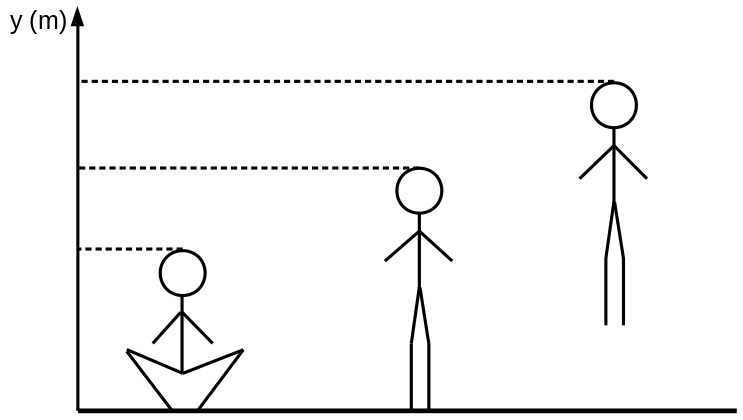
\includegraphics[scale=0.50]{figures/workPower/fig2.png}
\end{figure}

\pagebreak \clearpage

\input{momentum.tex}
\section{Torque}

\underline{\textbf{Part 1}} \par

\begin{verbatim}
https://phet.colorado.edu/sims/html/balancing-act/latest/balancing-act_en.html
Click "Game"
Complete all 4 levels - take screenshots of your results
\end{verbatim}

\underline{\textbf{Part 2}} \par

Background: it is well known that the harmonic series

\begin{equation}
\sum_{n=1}^{\infty} \frac{1}{n} = \frac{1}{1} + \frac{1}{2} + \frac{1}{3} + \frac{1}{4} + \dots
\end{equation}

aproaches infinity (albeit very slowly).
The similar sum

\begin{equation}
\sum_{n=1}^{\infty} \frac{1}{n^2} = \frac{1}{1^2} + \frac{1}{2^2} + \frac{1}{3^2} + \frac{1}{4^2} + \dots
\end{equation}

was first posed in 1650 and not solved until 1734 by Leonhard Euler.
Euler showed that this sum converges to $\pi^2$/6.

\vspace{\baselineskip}

Confirm Euler's result with the following experiment in Interactive Physics.
\begin{enumerate}
\item Create a beam of length 2 $m$ balanced at the center.
\item Put a 1 $kg$ mass 1 $m$ from the center, a 1/2 $kg$ mass 1/2 $m$ from the center, a 1/3 $kg$ mass 1/3 $m$ from the center, etc.
\item On the opposite edge of the beam, place a single mass. Decide what this mass should be to balance the system and explain how this confirms Euler's result.
\end{enumerate}

\begin{figure}[H]
\includegraphics[scale=0.50]{figures/torque/fig1.png}
\end{figure}

\pagebreak \clearpage

\input{angularKinematics.tex}
\input{orbits.tex}
\input{waves.tex}
\section{More Waves}

\underline{\textbf{Part 1}} \par

Choose reasonable values for velocity $v$, amplitude $A$, and wavelength $\lambda$ and reproduce the transverse traveling wave shown in lecture by using springs and masses in Interactive Physics.
Include several snapshots at different points in time.

\vspace{\baselineskip}

Tips: turn gravity off (optional); don't confuse the wave number $k$ with the spring constant $k_s$; consider the initial positions and velocities of each block.

\begin{figure}[H]
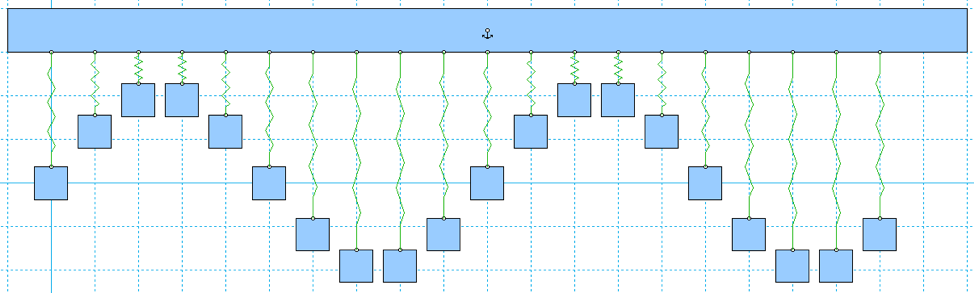
\includegraphics[scale=0.80]{figures/more-waves/fig1.png}
\end{figure}

Write down the function $f(x, t)$ that describes this wave and plot it in SageMath (see previous waves lab for examples).
Save the animated gif as part of your lab report.

\vspace{\baselineskip}

\underline{\textbf{Part 2}} \par

Create a standing wave in SageMath by summing together two traveling waves.
Save the animated gif as part of your lab report.


\pagebreak \clearpage

\input{dopplerEffect.tex}
\section{Electric Potential and Fields}

In this lab you will study the electric fields and potentials produced by different charge distributions and how charges respond to the presence of these fields.

\vspace{\baselineskip}

\underline{\textbf{Part 1}} \par
1. Consider placing two point charges on an x-y plane, the first charge, $q_1$, at $(x_1, y_1)$, and the second charge , $q_2$, at $(x_2, y_2)$.

\vspace{\baselineskip}

2. Derive an expression for the electric potential and field at any arbitrary point $(x, y)$ in terms of $q_1, q_2, x_1, x_2, y_1$ and $y_2$.

\vspace{\baselineskip}

3. Choose some reasonable values for $q_1, q_2, x_1, x_2, y_1$ and $y_2$ and make a rough sketch of what you expect the electric potential/field to look like.
Your picture doesn't necessarily have to be correct, but you should include some justification for why your sketch looks the way it does.

\vspace{\baselineskip}

4. Use SageMath to draw the exact electric potential and field using the expression derived above.
Below is an example.

\begin{verbatim}
x, y = var("x y")
g = Graphics()
g += contour_plot(1.5 + 0.2*x*y, (x, -4, 4), (y, -4, 4), fill=False, cmap='jet', labels=True, contours=[0, 1, 2, 3, 4], label_fontsize=14)
g += plot_vector_field((y/2, -x/2) , (x, -4, 4), (y, -4, 4)) 
g.show()
\end{verbatim}

Your final result should look something like the figure below.
Note how you can clearly see the two point charges at $(1, 2)$ and $(2, 1.5)$.

\begin{figure}[H]
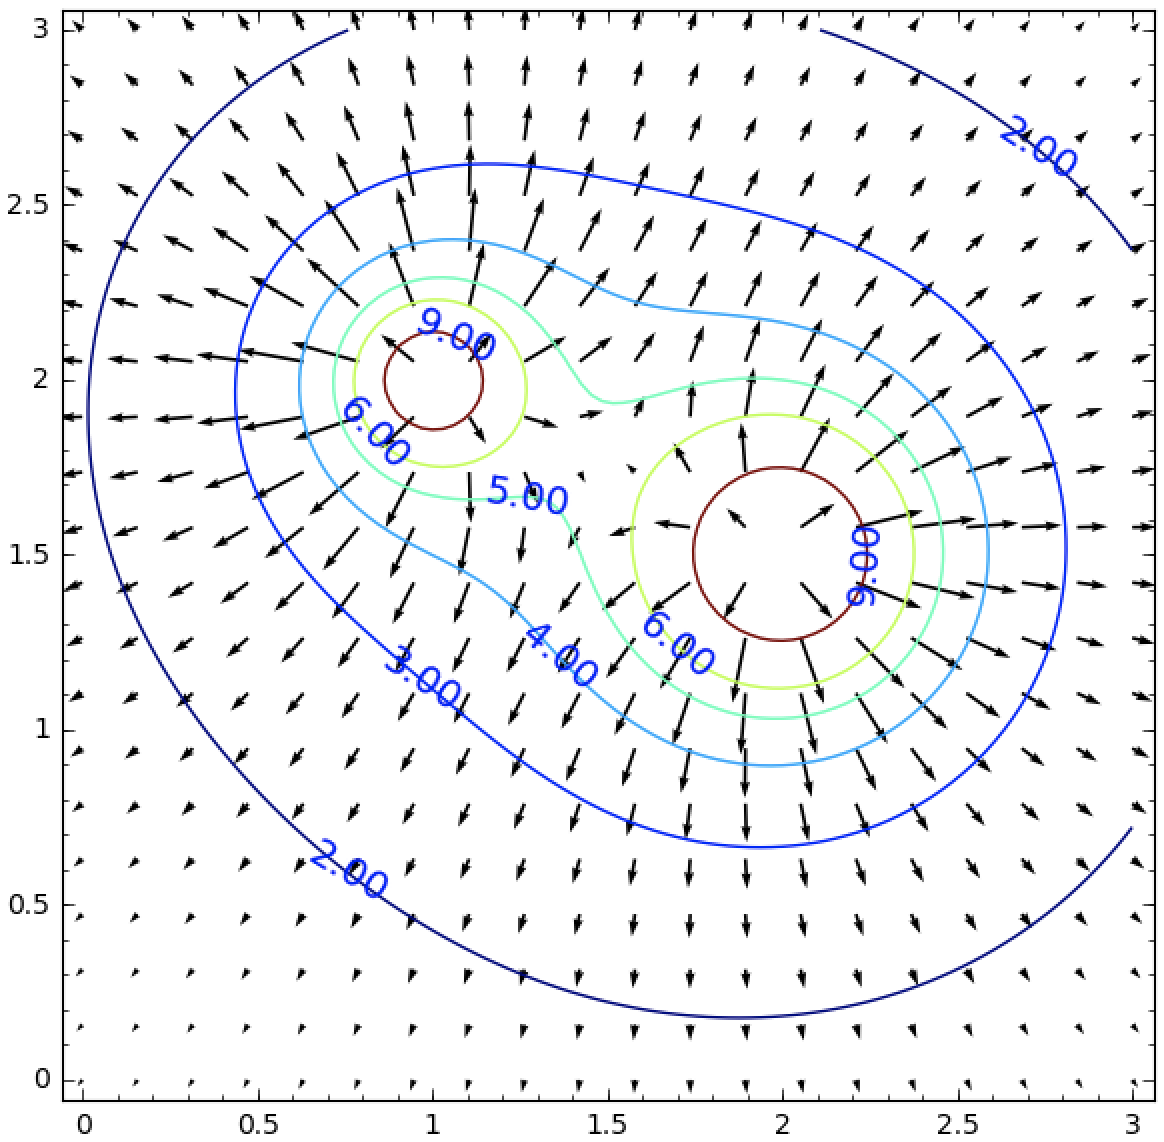
\includegraphics[scale=0.50]{figures/electric-potential-fields/fig1.png}
\end{figure}

\vspace{\baselineskip}

\underline{\textbf{Part 2}} \par

Go to http://www.physicsclassroom.com/PhysicsClassroom/media/interactive/Electric\%20Field\%20Hockey/index.html and complete levels 1, 2, 3, and 5.
Include screenshots in your lab report.

\pagebreak \clearpage

\section{Electric Flux and Path Integral}

\underline{\textbf{Part 1}} \par
Recall from class that when a point charge is located at the corner of a cube the electric flux through one of the opposite sides is $q / 24 \epsilon_0$.
Confirm this result (approximately) with the following procedure:

\begin{enumerate}
\item Divide the side of the cube into a 3x3 grid (as shown)
\item Calculate the electric field at the center of each grid square
\item Take the dot product of each of the 9 calculated electric fields with that grid square's area vector
\item Sum the 9 results above
\item Repeat with a 4x4 grid to show that more grid squares gives a better approximation to the exact result
\end{enumerate}

\begin{figure}[H]
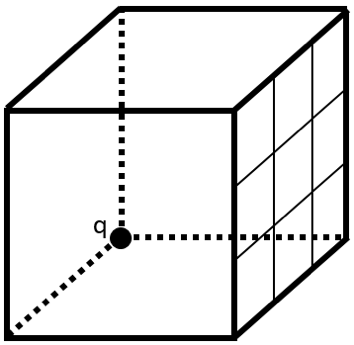
\includegraphics[scale=1.0]{figures/electric-flux-and-path-integral/fig1.png}
\end{figure}

\underline{\textbf{Part 2}} \par

See the figure below.
Calculate the change in electric potential between points A $(0, 1)$ and B $(2, 1)$ along the three paths shown.
Show all work!
Note that the two parts of path (1) are parallel and perpendicular to the electric field.
Extra credit (5\%): repeat for the path defined by the parabola $y = 2x^2 - 4x + 1$.

\begin{figure}[H]
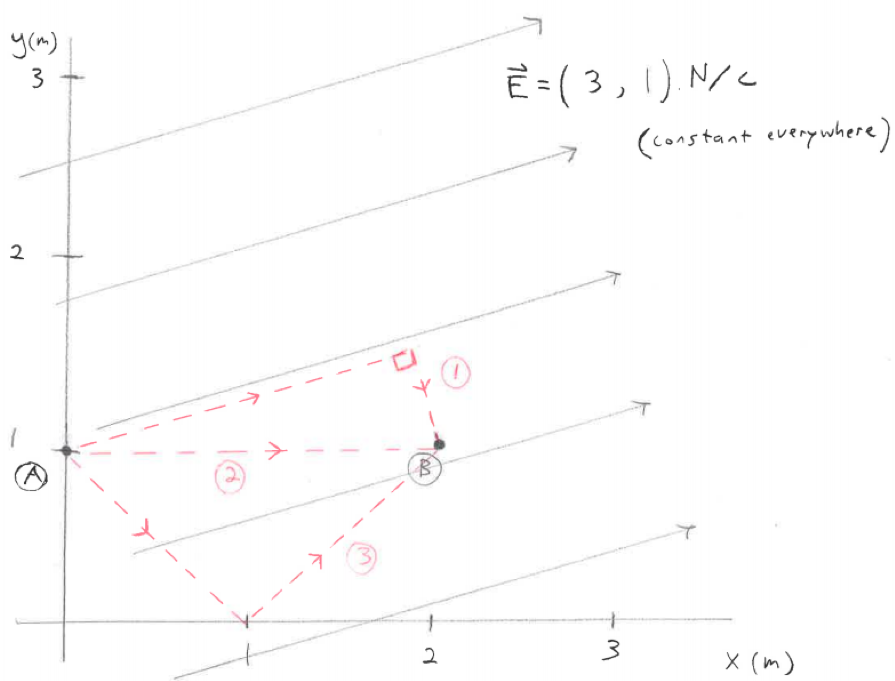
\includegraphics[scale=1.0]{figures/electric-flux-and-path-integral/fig2.png}
\end{figure}

\pagebreak \clearpage

\section{Electric Flux and Path Summations}

\underline{\textbf{Part 1}} \par
Recall from class that when a point charge is located at the corner of a cube the electric flux through one of the opposite sides is $q / 24 \epsilon_0$.
Confirm this result (approximately) with the following procedure:

\begin{enumerate}
\item Divide the side of the cube into a 3x3 grid (as shown)
\item Calculate the electric field at the center of each grid square
\item Take the dot product of each of the 9 calculated electric fields with that grid square's area vector
\item Sum the 9 results above
\item Repeat with a 4x4 grid to show that more grid squares gives a better approximation to the exact result
\end{enumerate}

\begin{figure}[H]
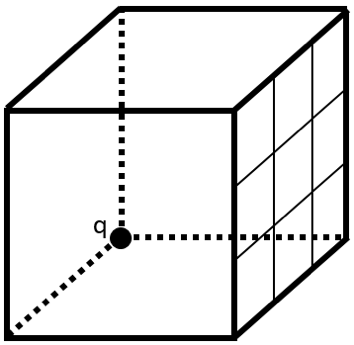
\includegraphics[scale=1.0]{figures/electric-flux-and-path-integral/fig1.png}
\end{figure}

\underline{\textbf{Part 2}} \par

See the figure below.
Calculate the change in electric potential between points A $(0, 1)$ and B $(2, 1)$ along the three paths shown.
Show all work!
Note that the two parts of path (1) are parallel and perpendicular to the electric field.
Extra credit (5\%): repeat for the path defined by the parabola $y = 2x^2 - 4x + 1$.

\begin{figure}[H]
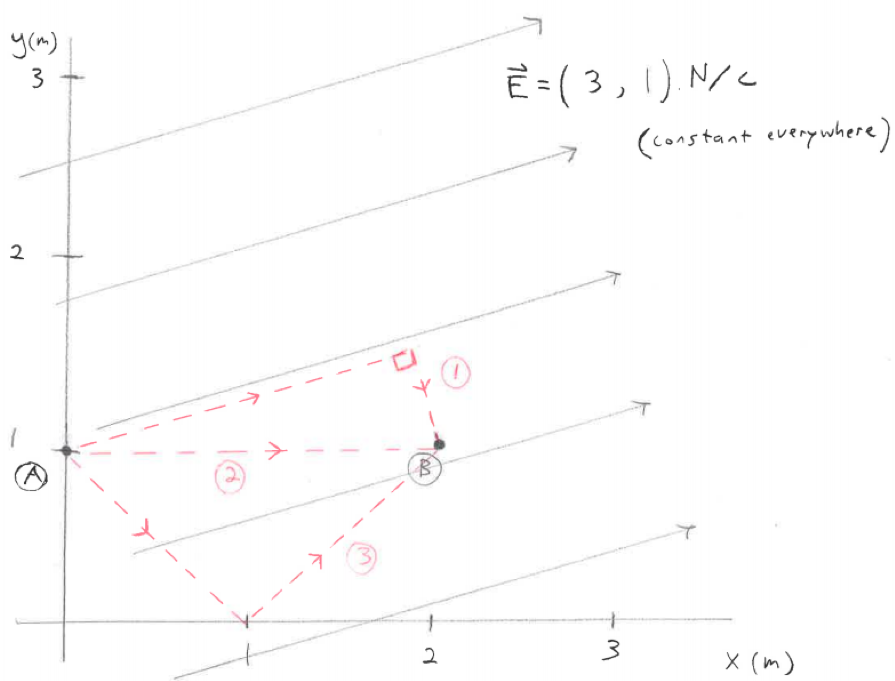
\includegraphics[scale=1.0]{figures/electric-flux-and-path-integral/fig2.png}
\end{figure}

\pagebreak \clearpage

\section{Resistor Circuits}

In this lab you will study the relationships between voltage, current, and resistance in simple DC circuits.

\vspace{\baselineskip}

Safety: electricity does have the ability to cause harm, but this lab should be very safe as long as you follow the instructions and don’t do anything stupid (e.g. take apart a power supply). 

\vspace{\baselineskip}

\underline{\textbf{Part 1}} \par
See https://phet.colorado.edu/sims/html/circuit-construction-kit-dc/latest/circuit-construction-kit-dc\_en.html for practice

\vspace{\baselineskip}

The DC power supplies at your lab stations are basically batteries with knobs so you can change the voltage.
Make sure your power supply is initially turned off (the switch may be in the back) and the knob is turned all the way down.
If it's not plugged in, plug it in and then turn it on and adjust the knob so the voltage is about 5V. 

\vspace{\baselineskip}

Take out your multi-meter and set it to voltage mode and measure the voltage of the power supply. It should read ~5V.

\vspace{\baselineskip}

The diagram below shows a standard breadboard layout:

\begin{figure}[H]
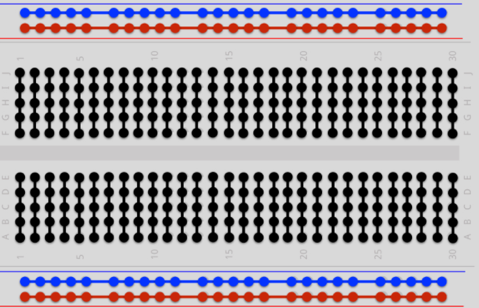
\includegraphics[scale=0.80]{figures/resistor-circuits/breadboard.png}
\end{figure}

The top 2 and bottom 2 rows (red (+) and blue (-)) are typically used for connecting to your power supply while the middle (black) is for plugging in circuit components.
Attempt to construct the following circuit:

\begin{figure}[H]
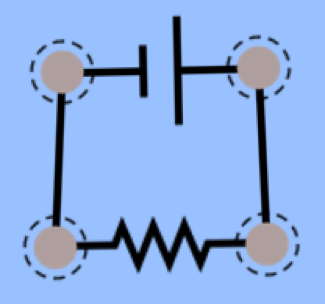
\includegraphics[scale=0.80]{figures/resistor-circuits/one-resistor.png}
\end{figure}

Have your instructor check your circuit before proceeding.
Next measure the voltage across the resistor and the current through the resistor.
Make sure your multi-meter is in the correct mode and that you connect it correctly.
Doing this incorrectly can blow a fuse in the multi-meter.
Note that measuring current requires you to break the circuit and put the meter in series with the resistor while measuring voltage requires you to put the meter in parallel with the resistor.
See below.

\begin{figure}[H]
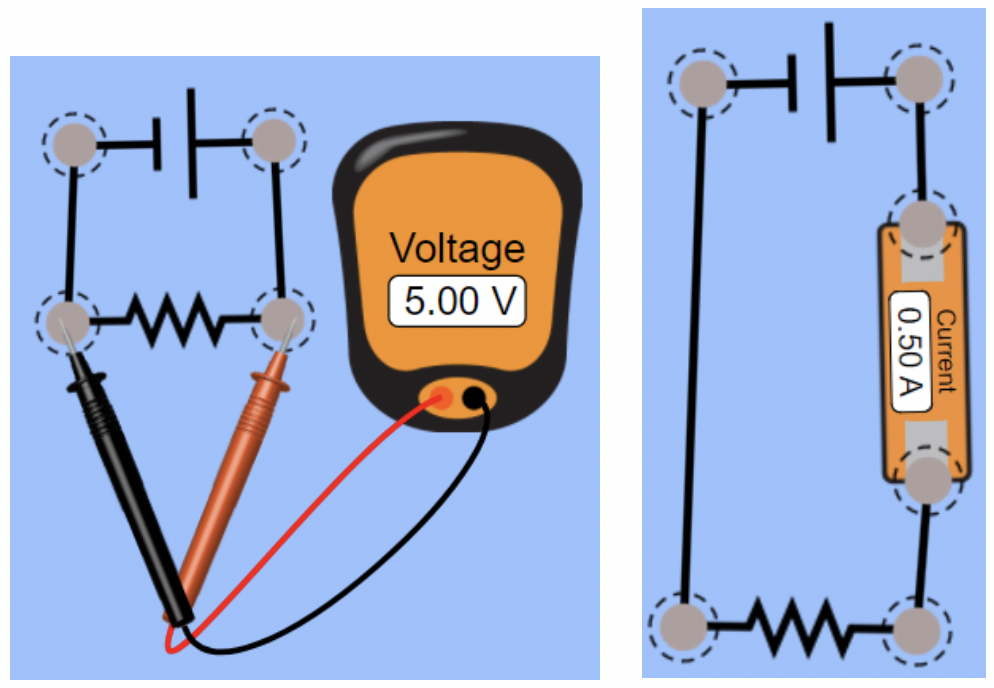
\includegraphics[scale=0.55]{figures/resistor-circuits/V-I-measurement.png}
\end{figure}

\underline{\textbf{Part 2}} \par

With your 5V power supply, construct the circuit below.
You may use your multi-meter to measure the resistance of the resistors rather than rely on the colored bands.
Calculate and then measure the voltage across and current through each resistor.
Also calculate and measure the equivalent resistance of the 3 resistor system.
Remember to be careful not to blow a fuse in the multi-meter!

\begin{figure}[H]
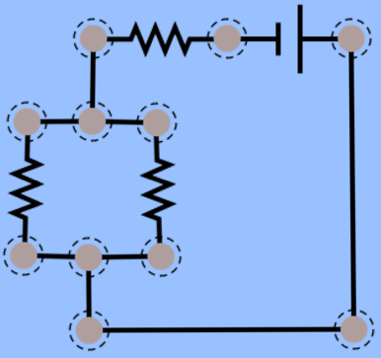
\includegraphics[scale=0.90]{figures/resistor-circuits/mixed-circuit.png}
\end{figure}

\pagebreak \clearpage

\section{Logic Circuits}

\underline{\textbf{Part 1 A}} \par

Build circuits consisting of a power supply, resistors, switches, and LEDs that obey the following logic: NOT, AND, and OR.
Make sure the current through any LEDs remains between 10 and 20 mA.
Safe values for voltage and resistance are approximately 2 $<$ V $<$ 4 V (DC) and 200 $<$ R $<$ 500 $\Omega$.  

\vspace{\baselineskip}

\underline{\textbf{Part 1 B}} \par

Construct a truth table for the 2-input, 2-output circuit shown below.

\begin{figure}[H]
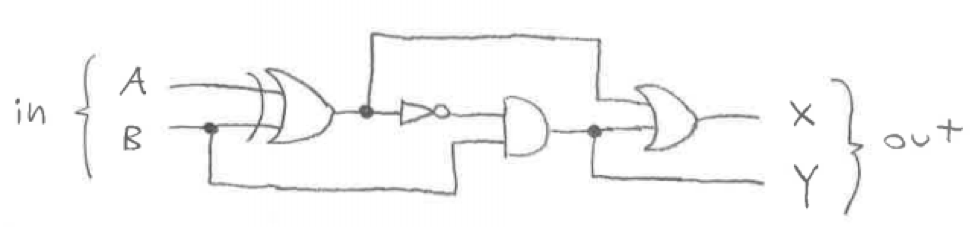
\includegraphics[scale=0.80]{figures/logic-circuits/fig1.png}
\end{figure}

\underline{\textbf{Part 2 A}} \par

Build NOT, AND, OR, and XOR circuits using a 4.5 V power supply, IC chips, resistors, and LEDs.
Note that the IC chips fit conveniently in the center of most breadboards as shown below and remember to use resistors in series with LEDs to keep the current between 10-20 mA.
Also note that a ``0'' input should be connected to ground (i.e. the negative side of your power supply), as opposed to being connected to nothing.
See the appendix for chip numbers.

\begin{figure}[H]
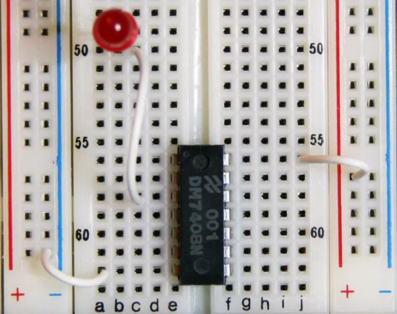
\includegraphics[scale=0.85]{figures/logic-circuits/fig2.png}
\end{figure}

Be very careful when removing the chips from the breadboards as the legs bend/break easily.
Avoid any unnecessary plugging and unplugging.
In order for the chips to function properly, pin 14 must be connected to +4.5 V and pin 7 must be connected to ground.
See below for pin numbers.

\vspace{\baselineskip}

The AND, OR, and XOR chips (below, left) each contain 4 gates while the NOT chips (below, right) contain 6 gates. 

\begin{figure}[H]
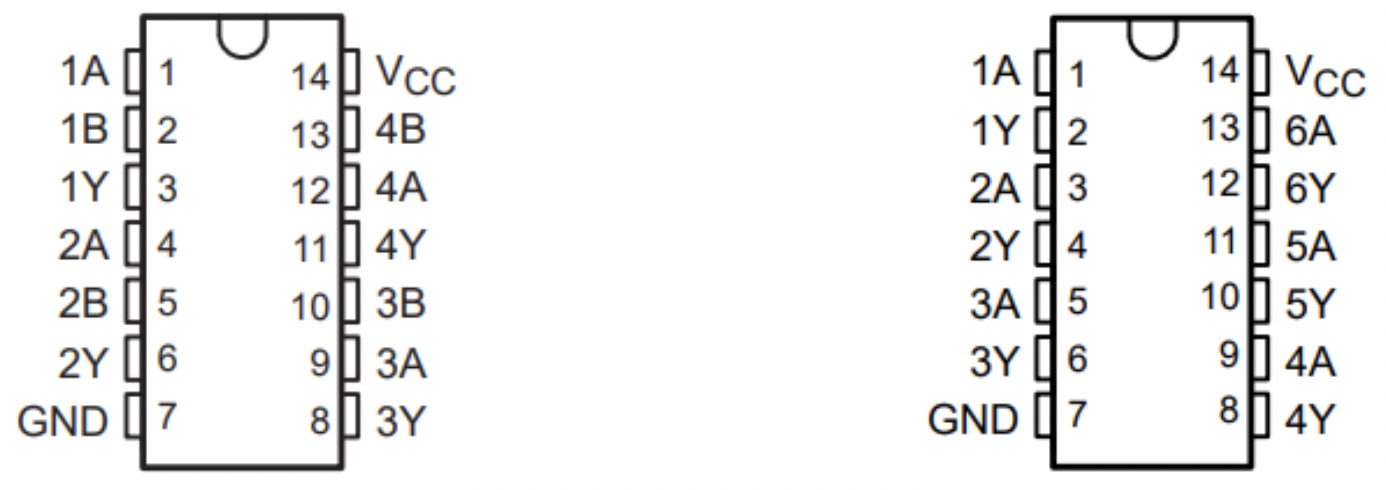
\includegraphics[scale=0.50]{figures/logic-circuits/fig3.png}
\end{figure}

In the above figures, A/B represent inputs and Y represents the output.
As an example, the figure below shows a more details picture of an OR chip.

\begin{figure}[H]
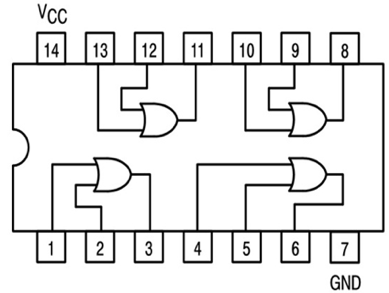
\includegraphics[scale=0.85]{figures/logic-circuits/fig4.png}
\end{figure}

\underline{\textbf{Part 2 B}} \par

Build the circuit below and confirm that it obeys XOR logic.

\begin{figure}[H]
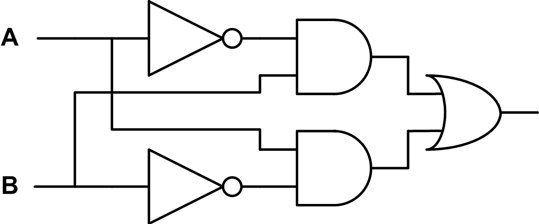
\includegraphics[scale=0.85]{figures/logic-circuits/fig5.png}
\end{figure}

\underline{\textbf{Part 2 C}} \par

Fill out the truth table for the following 2-input, 2-output circuit.
In the last column, consider XY a 2-digit binary number and convert it to decimal (i.e. base 10).
Build and test the circuit.
What did you just create?

\begin{figure}[H]
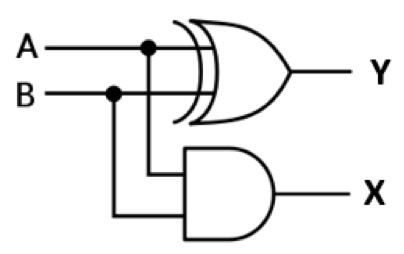
\includegraphics[scale=0.80]{figures/logic-circuits/fig6.png}
\end{figure}

\begin{tabular}[H]{ | c | c | c | c | c | }
\hline
A & B & X & Y & $\text{XY}_{10}$ \\
\hline
0 & 0 & \  & \  & \  \\
\hline
0 & 1 & \  & \  & \  \\
\hline
1 & 0 & \  & \  & \  \\
\hline
1 & 1 & \  & \  & \  \\
\hline
\end{tabular}

\vspace{\baselineskip}

\underline{\textbf{Appendix}} \par

\vspace{\baselineskip}

OR: 296-1615-5-ND/SN74HCT32N \\
XOR: 296-4777-5-ND/SN74AHCT86N \\
AND: 296-1606-5-ND/SN74HCT08N \\
NOT: 296-1605-5-ND/SN74HCT04N

\pagebreak \clearpage

\section{Biot-Savart Law}

In this lab you will build a small model that represents the magnetic field produced by a cicular loop of current.

\vspace{\baselineskip}

Let the loop have radius $a$, the current have magnitude $I$, and consider the field at a distance $x$ away from the loop's center along its symmetry axis as shown.

\begin{figure}[H]
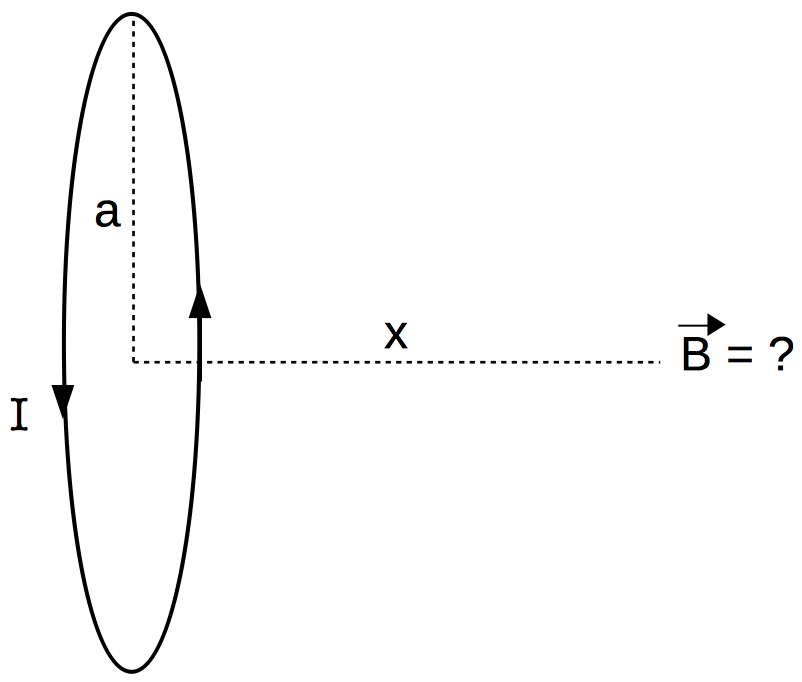
\includegraphics[scale=0.40]{figures/biot-savart/current-loop.png}
\end{figure}

If you consider the radius vectors connecting each small segment of the loop to the point of the field measurment, then a cone is formed.
Furthermore, according to the Biot-Savart Law, $d \vec{B} = \frac{\mu_0}{4 \pi} \frac{I d \vec{s} \times \hat{r}}{r^2}$, the fields produced by each small segment of the loop also form a second cone.

\begin{figure}[H]
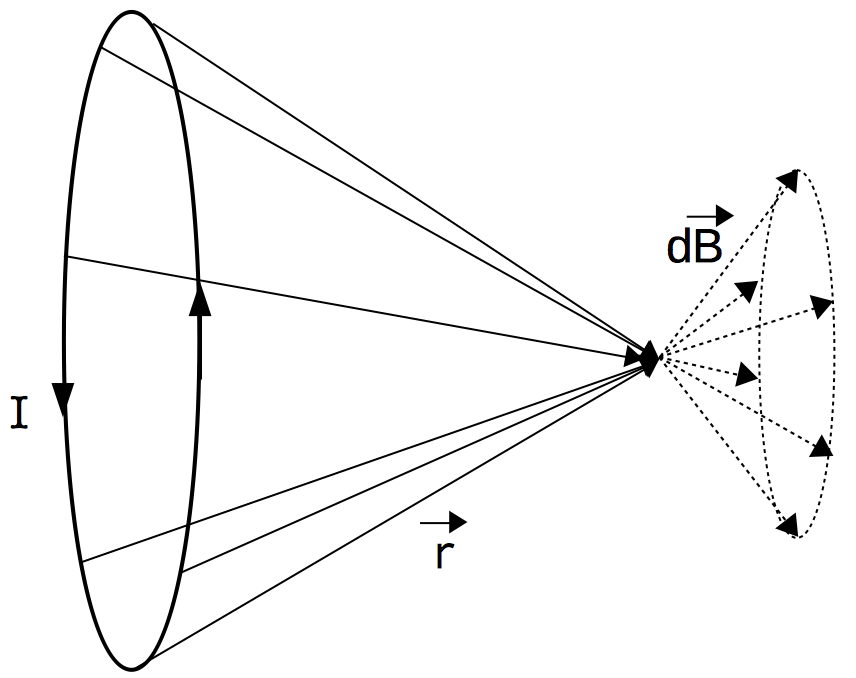
\includegraphics[scale=0.40]{figures/biot-savart/cones.png}
\end{figure}

Construct the two cone system above out of paper using the following technique.
First note that if you cut a straight line from the base of a cone to its tip and unroll the cone, you get a pacman shape (this is very similar to unrolling a cylinder and getting a rectangle).

\begin{figure}[H]
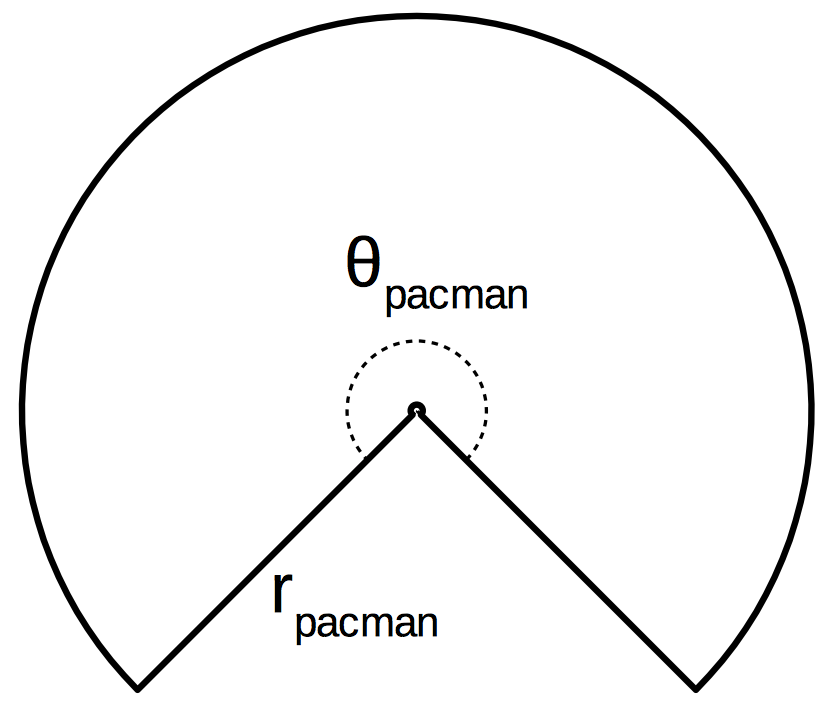
\includegraphics[scale=0.40]{figures/biot-savart/pacman.png}
\end{figure}

Solve for $\theta_{pacman}^{(1)}$, $r_{pacman}^{(1)}$, $\theta_{pacman}^{(2)}$, and $r_{pacman}^{(2)}$ in terms of $a$, $x$, and $h$, where the superscripts refer to the first and second cones and $h$ is the height of the second cone (measured from the center of its base to its tip).
The value of $h$ is arbitrary, it depends on how long you want the field lines to be.
For this lab, let $a = 4.6 \ cm$, $x = 6.3 \ cm$, and $h = 4.8 \ cm$.

\vspace{\baselineskip}

Once you've solved for $\theta_{pacman}^{(1)}$, $r_{pacman}^{(1)}$, $\theta_{pacman}^{(2)}$, and $r_{pacman}^{(2)}$, use a protractor and compass to draw the pacmen on paper, and cut them out.
Tape the pieces together and draw a few relevant vectors on the cones.
If you did everything correctly, the two cones should form $90^\circ$ angles with each other.

\begin{figure}[H]
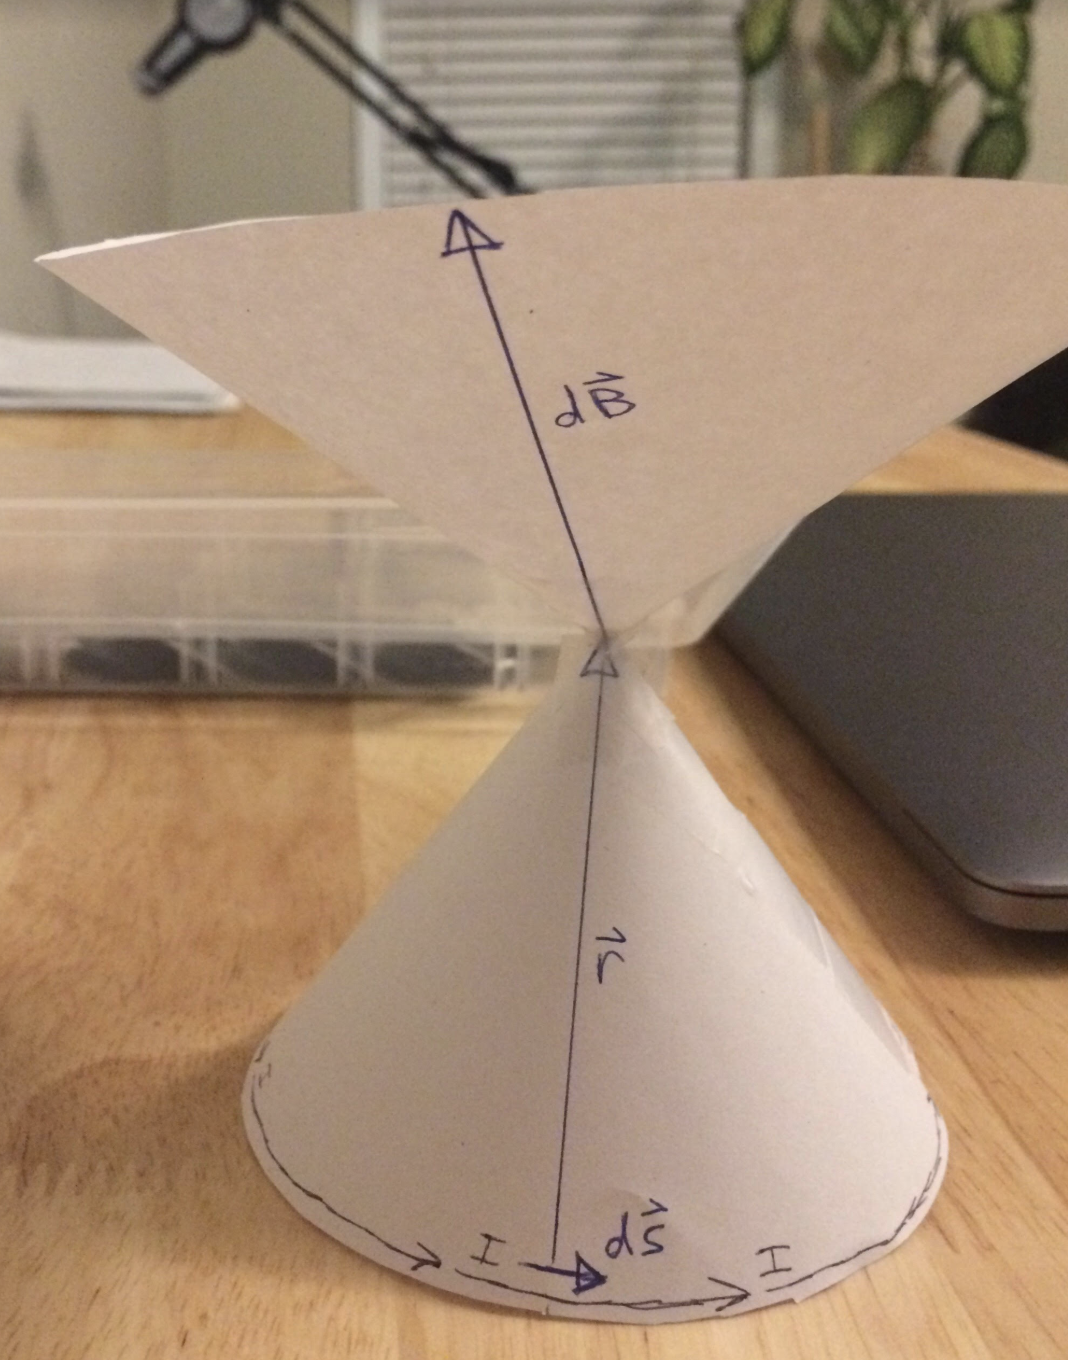
\includegraphics[scale=0.35]{figures/biot-savart/photo.png}
\end{figure}

\pagebreak \clearpage

\section{Stoke's Theorem and Divergence Theorem}

In this lab you will study the properties of the vector field
%
\begin{equation}
\label{eq:theVectorField}
\vec{v} = \frac{1}{\sqrt{0.2 + y^4 - 2xy^2 + x^2 + x^4 - 2x^2y + y^2}} \left[ \left(-y^2 + x \right) \hat{i} + \left( x^2 - y \right) \hat{j} + 0 \hat{k} \right]
\end{equation}
%
in the ranges $-2 < x < 2$, $-2 < y < 2$, $-2 < z < 2$ using Mathematica.
Begin by clearing any existing variables, defining the function, and defining variable ranges:
%
\begin{verbatim}
ClearAll["Global`*"];
denom[x_, y_] = Sqrt[0.2 + y^4 - 2*x*y^2 + x^2 + x^4 - 2*x^2*y + y^2];
vx[x_, y_] = (-y^2 + x)/denom[x, y];
vy[x_, y_] = (x^2 - y)/denom[x, y];
xmin = -2;
xmax = 2;
ymin = -2;
ymax = 2;
\end{verbatim}
%
Next, plot the vector field.
Since the field does not depend on $z$ and since the $z$-component is zero, a 2D plot will suffice.
Use VectorPlot and StreamPlot to get two different representations of the same function:
%
\begin{verbatim}
vp = VectorPlot[{vx[x, y], vy[x, y]}, {x, xmin, xmax}, {y, ymin, ymax}];
sp = StreamPlot[{vx[x, y], vy[x, y]}, {x, xmin, xmax}, {y, ymin, ymax}];
Grid[{{vp, sp}}]
\end{verbatim}
%
\begin{figure}[!h]
\centering
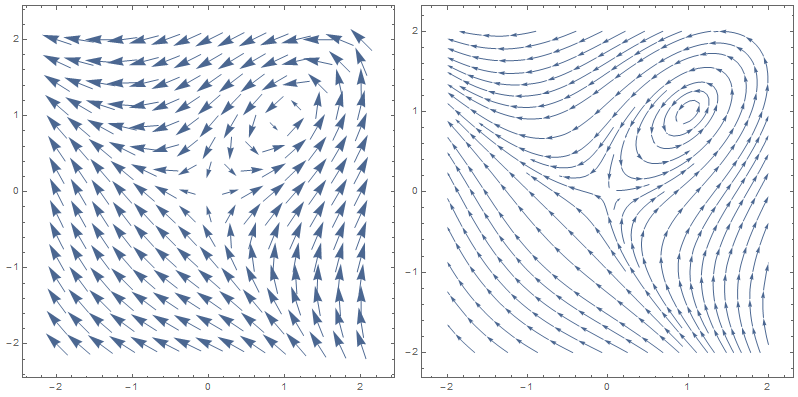
\includegraphics[scale=0.6]{figures/stokes-theorem/theVectorFieldPlots}
\caption{Plots of the vector field defined in equation~\ref{eq:theVectorField}.}
\label{fig:theVectorFieldPlots}
\end{figure}

\pagebreak

%%%%%%%%%%%%%%%%%%%%%%%%%%%%%%%%%%%%%%%%%%%
%%%%%%%%%%%%%%%%%%%%%%%%%%%%%%%%%%%%%%%%%%%

\underline{Part 1 - Stoke's Theorem}
\hfill \break

Stoke's Theorem states
%
\begin{equation}
\label{eq:stokesTheorem}
\oint_{Path} \vec{v} \cdot d\vec{s} = \int_{Surface} \left( \nabla \times \vec{v} \right) \cdot d\vec{A}.
\end{equation}
%
In this example, since the $z$-component of the field is zero, and since the field does not depend on z, Stoke's Theorem can be simplified to
%
\begin{equation}
\label{eq:stokesTheoremSimplified}
\oint_{Path} \vec{v} \cdot d\vec{s} = \int_{Surface} \left( \nabla \times \vec{v} \right)_z dA.
\end{equation}
%
Use Mathematica to calculate the curl of $\vec{v}$ (i.e. $\nabla \times \vec{v}$) and print out a few values at random points:
\begin{verbatim}
curlv[x_, y_, z_] = Curl[{vx[x, y], vy[x, y], 0}, {x, y, z}]
curlv[1, 1, 0]
curlv[1, 1, 0][[3]]
\end{verbatim}
notice that the $x$ and $y$ components of the curl of this vector field are zero.
Now make a plot of $\left( \nabla \times \vec{v} \right)_z$ as a function of $x$ and $y$ (remember, it doesn't depend on $z$):
\begin{verbatim}
dpz = DensityPlot[curlv[x, y, 0][[3]], {x, xmin, xmax}, {y, ymin, ymax},
	PlotLegends -> Automatic]
\end{verbatim}
%
\begin{figure}[!h]
\centering
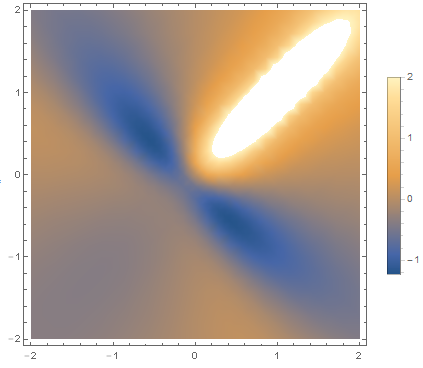
\includegraphics[scale=0.7]{figures/stokes-theorem/curlzDensityPlot.png}
\caption{$\left( \nabla \times \vec{v} \right)_z$}
\label{fig:curlzDensityPlot}
\end{figure}
%
and compare figures~\ref{fig:theVectorFieldPlots} and \ref{fig:curlzDensityPlot}.
Notice that the curl is large in the region where the field is ``curly.''

Create a grid in the $x$-$y$ plane and use a loop to get the value of the curl at the grid points:
\begin{verbatim}
nxdiv = 10;
nydiv = 10;
For[ix = 0, ix < nxdiv, ix++;
 For[iy = 0, iy < nydiv, iy++;
  xval = xmin + (ix - 0.5)*(xmax - xmin)/nxdiv;
  yval = ymin + (iy - 0.5)*(ymax - ymin)/nydiv;
  curlval = curlv[xval, yval, 0][[3]];
  vals = {xval, yval, curlval};
  Print[vals];
  ]] 
\end{verbatim}
and use these results to approximate the right hand side of equation~\ref{eq:stokesTheoremSimplified}.

Finally, use a similar technique to approximate the left hand side of equation~\ref{eq:stokesTheoremSimplified}.
For example:
\begin{verbatim}
(* ccw loop, starting at top right *)
nStepsPerSide = 20;
(* top: *)
For[i = 0, i < nStepsPerSide, i++;
 xval = xmax - (i - 0.5)*(xmax - xmin)/nxdiv;
 yval = ymax;
 vDotDs = vx[xval, yval]*(-1)*((xmax - xmin)/nStepsPerSide);
 Print[vDotDs];
 ]
(* left side: *)
For[i = 0, i < nStepsPerSide, i++;
 xval = xmin;
 yval = ymax - (i - 0.5)*(ymax - ymin)/nydiv;
 vDotDs = vy[xval, yval]*(-1)*((ymax - ymin)/nStepsPerSide);
 Print[vDotDs];
 ]
etc...
\end{verbatim}
Once your program is fully written and debugged, increase $nxdiv$, $nydiv$, and $nStepsPerSide$ to $100$ to improve your accuracy.
Confirm Stoke's Theorem by comparing your two calculated numbers.

%%%%%%%%%%%%%%%%%%%%%%%%%%%%%%%%%%%%%%%%%%%
%%%%%%%%%%%%%%%%%%%%%%%%%%%%%%%%%%%%%%%%%%%

\hfill \break
\underline{Extra Credit - The Divergence Theorem}
\hfill \break

Use a similar approach to confirm the Divergence Theorem for this same vector field.

\pagebreak \clearpage

\section{Path of Least Time}

Consider a situation in which you have to rescue a drowning friend.
You want to get to him in the least amount of time, and since your velocity on land is larger than your velocity in water your path may not necessarily be a straight line. 
(This is an analogy for how light travels.)

\vspace{\baselineskip}

Part A - Derive a formula for finding the path of least time.

\vspace{\baselineskip}

Part B - Experimentally confirm your equation using the simulation found here: https://github.com/naharrison/path-of-least-time/releases

\vspace{\baselineskip}

Follow the instructions on that site to open the simulation – make sure to actually extract the files from the zip file.
Right-click to run/restart the simulation; left-click to move the 3 points of interest.
The relevant data will be printed to the screen in the following order:

\vspace{\baselineskip}

Starting point x

Starting point y

Transition point x

Transition point y

End point x

End point y

Elapsed time

\vspace{\baselineskip}

Note that the unit of distance is pixels and the unit of time is ms.
The velocity on land is 0.06 px/ms and the velocity in water is 0.015 px/ms. Also note that the origin is in the top left of the screen.


\pagebreak \clearpage

\section{Chaos}

In this lab you will study some interesting properties of chaotic systems.

\vspace{\baselineskip}

\underline{\textbf{Part 1}} \par
Draw 3 points on a piece of paper to form a triangle.
Label the points 0, 1, and 2.
Also randomly draw a 4th point - this will be the starting point of the experiment.
Next, randomly generate either a 0, 1, or 2 (e.g. by rolling dice), the number generated will correspond to one of the corners of the triangle.
Make a new point halfway between the starting point and the corner of the triangle selected in the previous step; this point becomes the new starting point for the next iteration.
Repeat this process of making new points halfway between the last point and the corner of the triangle randomly selected many times.

\vspace{\baselineskip}

Do at least 10 points by hand until you get the idea.
Your final result should contain at least 2000 points.
If you are a student who insists that learning basic coding is not useful then you can do all 2000 points by hand.
Otherwise, try the following SageMath script.

\begin{verbatim}
# Create a graphics object to display the points
g = Graphics()


# Add 3 points that make up a triangle
tri = [ (1, 1), (3, 1), (2, 3) ]
g += point(tri, color="red", size=35)


# Choose a random starting point
x = 2.6 
y = 1.3 
g += point((x, y), color="black", size=10)


# Generate random numbers (0, 1, or 2)
# corresponding to points on the triangle.
# For each iteration, move halfway from the 
# last point to the chosen triangle point.

nPts = 2500
for i in range(0, nPts):
  rand = ZZ.random_element(0, 3)
  x = x + 0.50*(tri[rand][0] - x) # experiment with the fraction
  y = y + 0.50*(tri[rand][1] - y) # experiment with the fraction
  g += point((x, y), color="black", size=10)


g.show()
\end{verbatim}

% some interesting results:
% 0.25 total randomness
% 0.5 perfect fractal pattern
% 0.8 3 groups of 3 groups of 3 groups

% TODO Add barnsley fern example

\pagebreak \clearpage

%%  hyp_a = 0.8 # x-intercept of hyperbola
%%  hyp_c = 1.2 # x-value of hyperbola focal point
%%  
%%  ell_b = 1.5 # length of short radius for ellipse
%%  ell_c = 2.1 # distance between center and focal point for ellipse
%%  ell_th = 0.5 # theta rotation angle (radians) of ellipse (ccw)
%%  ell_a = sqrt(ell_b^2 + ell_c^2)
%%  
%%  # want the left focal point of the ellipse to match the left focal point of the hyperbola:
%%  ell_x = ell_c*cos(ell_th) - hyp_c # ellipse center x
%%  ell_y = ell_c*sin(ell_th) # ellipse center y
%%  
%%  ell_rfx = ell_x + ell_c*cos(ell_th) # ellipse right focal point x
%%  ell_rfy = ell_y + ell_c*sin(ell_th) # ellipse right focal point y
%%  ell_lfx = ell_x - ell_c*cos(ell_th) # ellipse left focal point x
%%  ell_lfy = ell_y - ell_c*sin(ell_th) # ellipse left focal point y
%%  
%%  var('x y')
%%  xmin = -2.5
%%  xmax = 3.5
%%  ymin = -1.5
%%  ymax = 3.5
%%  
%%  hyp = (x^2)/(hyp_a^2) - (y^2)/(hyp_c^2 - hyp_a^2) == 1
%%  hyp_plot = implicit_plot(hyp, (x, xmin, xmax), (y, ymin, ymax), color="red")
%%  
%%  ell = (((x - ell_x)*cos(ell_th) + (y - ell_y)*sin(ell_th))^2)/(ell_a^2) + (((x - ell_x)*sin(ell_th) - (y - ell_y)*cos(ell_th))^2)/(ell_b^2) == 1
%%  ell_plot = implicit_plot(ell, (x, xmin, xmax), (y, ymin, ymax))
%%  
%%  g = Graphics()
%%  g += hyp_plot
%%  g += ell_plot
%%  g += point((-hyp_c, 0), size=35, color="red", alpha=0.5)
%%  g += point((hyp_c, 0), size=35, color="red", alpha=0.5)
%%  g += point((ell_x, ell_y), size=35, alpha=0.5)
%%  g += point((ell_rfx, ell_rfy), size=35, alpha=0.5)
%%  g += point((ell_lfx, ell_lfy), size=35, alpha=0.5)
%%  g.show()

\section{Optics - Mirrors}

In this lab you will study the reflective properties of curved mirrors.

\hfill \break
\underline{Part 1 - Hyperbolic Mirrors}
\hfill \break

Consider the hyperbola
%
\begin{equation}
\label{eq:hyperbolaEq}
\frac{x^2}{0.8^2} - \frac{y^2}{1.2^2 - 0.8^2} = 1
\end{equation}
%
shown if figure~\ref{fig:hyperbolaPlot}.
Choose a light ray originating from the right-most region of the plot and heading towards the left focal point.
Show mathematically that when this ray is reflected by the hyperbolic mirror, it will pass through the second focal point.
Use a ruler to \textit{accurately} draw the path of this ray, stopping at the second focal point.
Draw the path for at least two more rays that are also initially headed towards the left focal point.
%
\begin{figure}[!h]
\centering
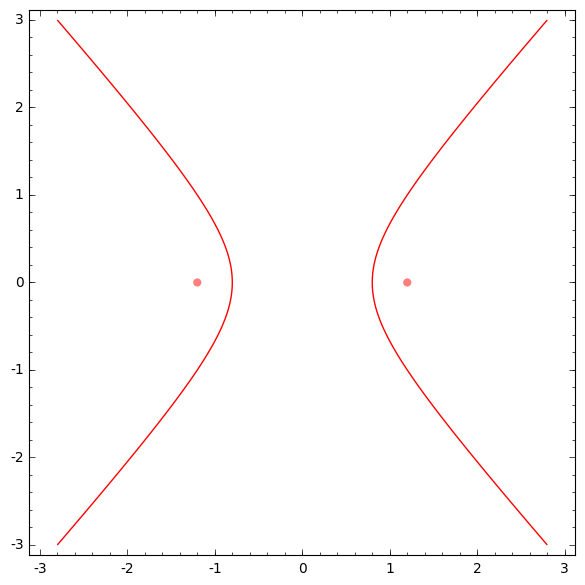
\includegraphics[scale=0.85]{figures/optics-mirrors/hyperbolaPlot.png}
\caption{The hyperbola defined in equation~\ref{eq:hyperbolaEq}.}
\label{fig:hyperbolaPlot}
\end{figure}

%%%%%%%%%%%%%%%%%%%%%%%%%%%%%%%%%%%%
%%%%%%%%%%%%%%%%%%%%%%%%%%%%%%%%%%%%

\hfill \break
\underline{Part 2 - Elliptical Mirrors}
\hfill \break

Consider the ellipse
%
\begin{equation}
\label{eq:ellipseEq}
\frac{x^2}{1.5^2 + 2.1^2} + \frac{y^2}{1.5^2} = 1
\end{equation}
%
shown if figure~\ref{fig:ellipsePlot}.
Choose a light ray originating from the right-most focal point.
Show mathematically that when this ray is reflected by the elliptical mirror, it will pass through the second focal point.
Use a ruler to accurately draw the path of this ray, stopping at the second focal point.
Draw the path for at least two more rays that also originate from the right-most focal point.
%
\begin{figure}[!h]
\centering
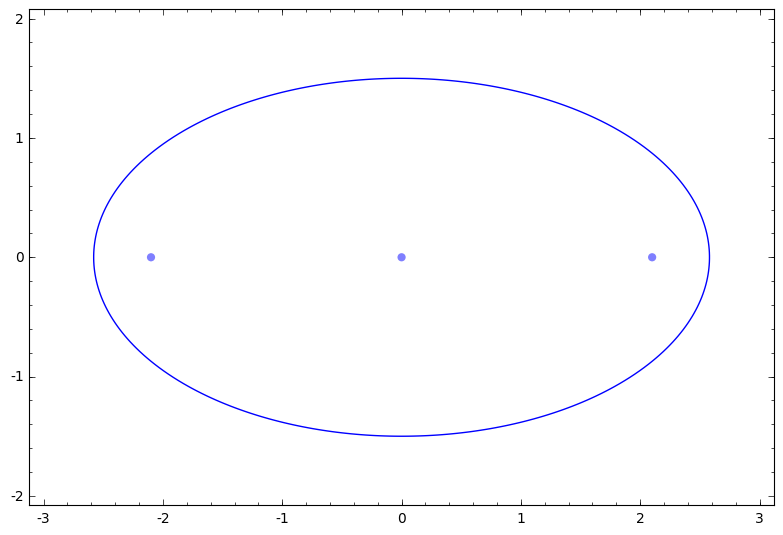
\includegraphics[scale=0.85]{figures/optics-mirrors/ellipsePlot.png}
\caption{The ellipse defined in equation~\ref{eq:ellipseEq}.}
\label{fig:ellipsePlot}
\end{figure}

%%%%%%%%%%%%%%%%%%%%%%%%%%%%%%%%%%%%
%%%%%%%%%%%%%%%%%%%%%%%%%%%%%%%%%%%%

\hfill \break
\underline{Part 3 - Mirror Combinations}
\hfill \break

As shown in figure~\ref{fig:both}, an ellipse and hyperbola share a focal point (left-most point).
Use a ruler, plus the rules of reflection from parts 1 and 2, to accurately draw the location where all\footnote{consider only rays that hit the ellipse first} rays originating from the right-most point intersect.
%
\begin{figure}[!h]
\centering
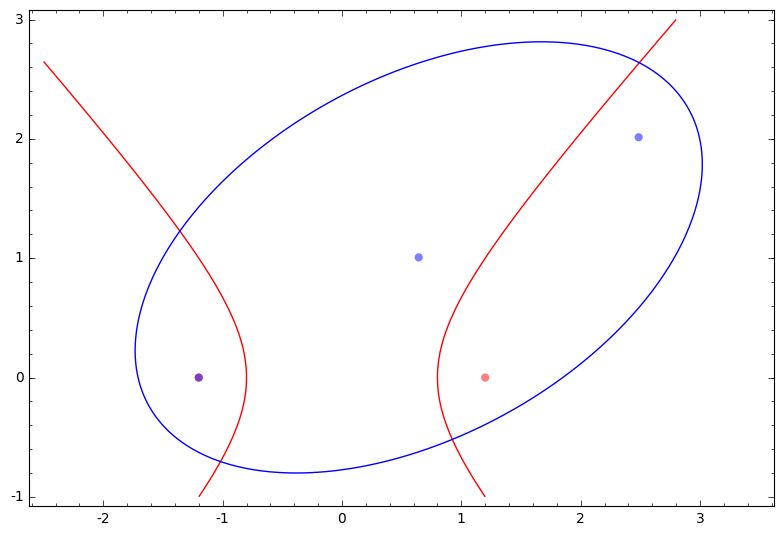
\includegraphics[scale=0.85]{figures/optics-mirrors/both.png}
\caption{An ellipse and a hyperbola sharing a focal point.}
\label{fig:both}
\end{figure}

\pagebreak \clearpage


\end{document}
